\section{Introduction}
\label{sec:introduction}

Climbing has become a popular sport during the last decades \autocite{freizeitklettern}. According to the international Federation of Sport Climbing (iFSC),  there are actually over 25 million active sport climbers worldwide \autocite{IFSC:figures}. As other sports, climbing includes improving motor skills, strength, endurance, knowledge, etc. \autocite{Kajastila:2014}. Therefore, professional training consists of repetition cycles, during which an experienced trainer observes a trainee and gives feedback by commenting on movements \autocite{Ladha:2013:CSA:2493432.2493492}. Occasionally, video analysis is used to assist this process, which is rather cumbersome, though, and remains restricted to observation of the what was visible to the camera. Research looking into the climbing movements that is concerned with new training approaches still is an emerging discipline with high potential, \cf \ref{appendix:interview_f_d}.

In this work, it is investigated how trainers coach their trainees and how this process can be supported by using technology. Therefore, trainers were interviewed concerning their training methods. Based on their statements, two concepts have been developed: Providing climbers with a live video of themselves while climbing, and providing climbers with a replay of their movements performed by a 3D avatar. Both approaches have been tested in a small perception study and were received well, though, the benefit of the live video is questioned more critically than the benefit of the replay in 3D.

\section{Related Work}

Various approaches using technology-related to the training process for climbing have been tested so far, for example \textcite{Cha2015} analyzed full body motions using a Microsoft Kinect and \textcite{Kajastila:2014:ACI:2611780.2581139} transformed climbing walls into interactive surfaces. In \citeyear{weikersdorfer2016tracking}, \textcite{weikersdorfer2016tracking} successfully used three cameras to capture boulder movements and reproduced them in a 3D model.

Wearables have also been used for analyzing various aspects of climbing: Starting in \citeyear{Ladha:2013:CSA:2493432.2493492}, \textcite{Ladha:2013:CSA:2493432.2493492} introduced a wrist strap for assessment of climbing activities. Two years later \textcite{Kalyanaraman:2015:ARC:2800835.2800856} suggested an approach for \citetitle{Kalyanaraman:2015:ARC:2800835.2800856}. In early \citeyear{Kosmalla:2016:CIP:2858036.2858562}, \textcite{Kosmalla:2016:CIP:2858036.2858562} tested wearables with different output signals for their perception and later that year \textcite{Schulz:2016} examined how well Myo Gesture Control Armbands are suitable to distinguish different grab motions.

There are other approaches which are not directly related to climbing analysis. Both \textcite{Goldman:2008:VOA:1449715.1449719} and \textcite{Dragicevic:2008:VBD:1357054.1357096} suggested a novel approach on video navigation using direct interaction with the video rather than a traditional slider, which allows a more intuitive navigation through space and time.

\section{Systematic Training for Sport Climbing}

As climbing has evolved over time, the need for systematic training in this sport arose. Originally, climbing was reserved to an adventurous group of locals living close to mountains and was a necessary part to reach mountaintops, which were otherwise impossible to summit. Today it has become a sport with a huge variety, which is easily accessible for many people. Although some still exercise climbing in its original form, most people practice \textit{sport climbing,} which is more focused on the athletic aspect and physical exercise \autocite{Kosmalla:2016:CIP:2858036.2858562}. Sport climbers go up routes on natural rock faces or on artificial climbing walls reaching a height up to \SI{40}{\m}. The goal is reaching the end of a route using nothing but the given hand- and footholds to hold onto or stand upon, respectively. The difficulty is determined by the nature of the hand- and footholds and the overall slope of the face.

With the rise of competitive climbing, systematic training became part of the sport \autocite{billat1995energy, horst2016training}, which includes trainers teaching others how to climb. The first goal of this work was to comprehend how trainers coach their trainees. Therefore, climbing coaches were interviewed regarding their training methods. The following sections explain where the ideas originated which were tested later during this work and how they relate to the interview statements.

\subsection{Interviewing Coaches}

In preparation of this study, a total of three interviews has been conducted. They were held openly with only a few prepared questions regarding their experience with using technology throughout training sessions. This way the interview partners could explain their motivation, their understanding of the sport, and the impact this has on their teaching methods. The summarized interviews can be found, \cf \secref{appendix:interview_f_d} to \secref{appendix:interview_f_l}.

One of the main themes reoccurring in all three interviews is the responsibility of the trainer. It is their unanimous opinion, that a trainer must be able to spot deficits in their trainees' performances, precisely name and explain them, and provide methods for working on them. They emphasize how highly individual climbing is and that it requires customized mentoring. Furthermore, IL and FL point out the importance of the right balance of climbing on high walls with harnesses and ropes, and on low walls without rope, called \enquote{bouldering}, for an efficient training. The latter accounts for \SI{80}{\percent} of the training time since it is highly intensive and it allows for corrective actions more easily.

All of the three interviewed trainers had previously worked with video analysis. They used their smartphones with apps like Technique\footnote{\url{http://www.hudl.com/products/technique}} or Coach's Eye\footnote{\url{https://www.techsmith.de/coachs-eye.html}} to record videos of trainees. Meanwhile FD and IL mainly use the recordings for immediate feedback, FL rather looks through the material post hoc and writes detailed analysis. One of the drawbacks of video analysis mentioned in the interviews, is the limited range that can be covered. When the trainee climbs up meanwhile the camera operator stays on the ground, the lower body of the climber increasingly obstructs the upper body. In order to overcome this problem, the camera operator would have to move further away, which again is not always possible and may result in worse video quality, especially when zooming in with a smartphone.

FL further reveals he has found out that the improvement video analysis offers for solving difficult moves is negligible. For him it is important that athletes are able to verbalize what went wrong. This he tries to teach them by encouraging them to characterize and even write down the description their pose, \eg right before they fell off the wall. Going through this process repeatedly causes an enhanced sense of their own bodies for the athletes. This is the basis for efficient climbing since it allows them to anticipate moves and plan them strategically while still on the ground, and more importantly before actually performing them. FL refers to this process of imagining oneself doing something without actually doing it as the well known practice of imagery.

\subsection{Ideas for Complementary Training Methods}
\label{sec:ideas}

Previous to the interviews, ideas were gathered on how technology might be used to support climbers. Most ideas had in common that they involved either video or some other form of recording climbing movements. The following is a discussion of these ideas against the backdrop of the interviews conducted in the meantime. 

One group of ideas addresses the enhancement of the video playback. Based on the concepts of \textcite{Goldman:2008:VOA:1449715.1449719} and \textcite{Dragicevic:2008:VBD:1357054.1357096}, navigating through a video of someone climbing up a wall could be detached from the timeline and additionally include the recorded wall itself. By tapping on a point of interest in the wall seen in the video, the video would skip to the frame where the climber is near that position in the wall. Expanding on that, moving through the video would also be possible by dragging limbs of the climber to a position in the image and thereby to a frame of interest. Additionally, the climber could be overlayed with visual guidelines, \eg indicating its center of gravity.

The second group of ideas revolves around dimensions being recorded. Regular video analysis works with 2D images which do not allow a change of perspective afterwards. Depending on the quality of the footage, reconstructing the pose of an athlete from it might be imprecise. A recording of movements mapped to a 3D model of joints in a skeleton would allow for a more precise replay of those movements. Further it allows a change of perspective afterwards, which makes it easier to reveal details that would otherwise be hard to spot, \eg the position of a hand covered by the upper body.

The third group of ideas is about live video feedback. Instead of providing an athlete with a video recording after performing a task, a live video is provided to the athlete -- trough a pair of smart glasses -- while performing a task. Assuming that a trainer is still on the ground next to a camera operator, the trainer can comment on the athletes performance, and the athlete can immediately take the visual perspective using the live video broadcast by the camera operator. Sharing the same visual perspective, may reduce misunderstandings between trainer and trainee. Furthermore, the visual perspective the athlete is provided with, looking up standing on the ground, is actually the same from which the athlete has to plan routes using imagery. Hence this method might have a positive effect on body awareness and on movement anticipation skills.

\paragraph{Picking Ideas to Evaluate}

Out of these three groups of ideas, a subset of ideas has been extracted to be tested. Acting on the importance ascribed to body awareness and imagery, the first group has been entirely discarded, since the expected impact on these skills was low. The same applies to  the expected benefit from additional overlays in video recordings. In contrast to group one, the remaining groups appeared more promising. Both add novel input supporting the mental recap of movements, which is why their core concepts should be evaluated for  their perception and acceptance in a small study.

\section{Perception Study}

To gain a coarse overview on how the two ideas introduced in \secref{sec:ideas} are received, a small preliminary study was conducted in a local climbing gym. The goal was to find out if any of these ideas might be worth looking into more deeply.

\subsection{Method}
\paragraph{Pariticipants}

Six climbers (2 female, 4 male) participated in the study. Their age ranged from 17 to 41, with an average of  28.7 years ($\sigma = 9.6$). All participants are members of a training group, which meets twice a week. All of them climb lead, that is without a rope coming from above. When asked for their on-sight level --- the difficulty they climb successfully without falling or resting supported by the rope --- all stated to climb an UIAA $5+$ or harder ($6 \pm$ half a degree).
\paragraph{Conditions}

Two methods of visual movement examination were tested for their user perception and acceptance. The first condition consisted of a live video, showing the participant from behind which was shown to the participant through a pair of smart glasses. A motion capture suite was used to record movements for post hoc examination as second condition. 
\paragraph{Tasks}

On the one hand, climbing is psychologically and physically stressful for a climber, especially when climbing close to the physical limit. On the other hand, challenging trainees to perform a move which they consider impossible puts them under stress at first, yet achieves a great learning effect once they manage to do it anyways. Therefore, the routes to climb or even just single moves were picked individually to be appropriate for each participant.
\paragraph{Design}

The experiment was designed in a way that all of the participants had a to perform two moves of mixed difficulty under the first condition. Only a two of the participants tested the second condition, but the order in which they tested the first and the second condition was random.
\paragraph{Procedure}

First, each participant was given an introduction during which the experimenter explained the idea of imagery, the upcoming tasks, as well as the condition that was to be tested. Before actually climbing, the participants were questioned regarding age, gender and climbing experience. For the first condition, they were then handed the smart glasses and assisted in putting them on, so they can fully see the display. The second condition required helping them getting into the motion capturing suite and initializing it. Once the participants were set up, they were given a task and began to climb. While climbing, participants were either asked to think aloud or the experimenter asked questions regarding their experience with the system right at that moment. Meanwhile, the camera operator stood on the ground, moving around to capture each participant from an optimal angle.

A final questionnaire --- an adapted version of the System Usability Score (SUS), which assessed to overall experience of the system used --- was handed to the participants. In total, six participants tested the first condition and two tested the second condition, where each run took about \SI{10}{\min} for the first condition and up to \SI{60}{\min} for the second condition, involving the motion capture suite.
\subsection{Apparatus}

Testing the idea of live video required a setup which enables athletes to see a live video of themselves climbing while climbing. This video would come from a camera, operated by a second person standing on the ground and would be transmitted to the athlete on the wall, \cf \figref{fig:live-video-action}. Since there is no solution for this available off the shelf, a custom solution had to be crafted which fulfilled the following requirements: \textit{Minimally Invasive:} Like when recorded on video for a regular video analysis, athletes should not be limited by the system in any way and be able to climb up the wall as usual. \textit{Low Latency:} Climbers should  perceive every movement immediately in the live video. \textit{Easy Setup:} The setup should not last longer than putting on climbing shoes to keep inhibitions of using the system low.

\begin{figure}[h]
    \centering
    \begin{subfigure}[t]{0.49\columnwidth}
        \centering
        \begin{overpic}[width=\textwidth]{figures/images/Google-Glass.jpg}
          \rbox{-1}{1}{\textcolor{source}{\tiny{Source: \href{https://de.wikipedia.org/wiki/Datei:Google_Glass_Main.jpg}{Wikipedia}}}}
        \end{overpic}
        \caption{A model of the Google Glass similar to the one used in the experiment.}
        \label{fig:google-glass}
    \end{subfigure}
    \hspace*{\fill}
    \begin{subfigure}[t]{0.49\columnwidth}
        \centering
        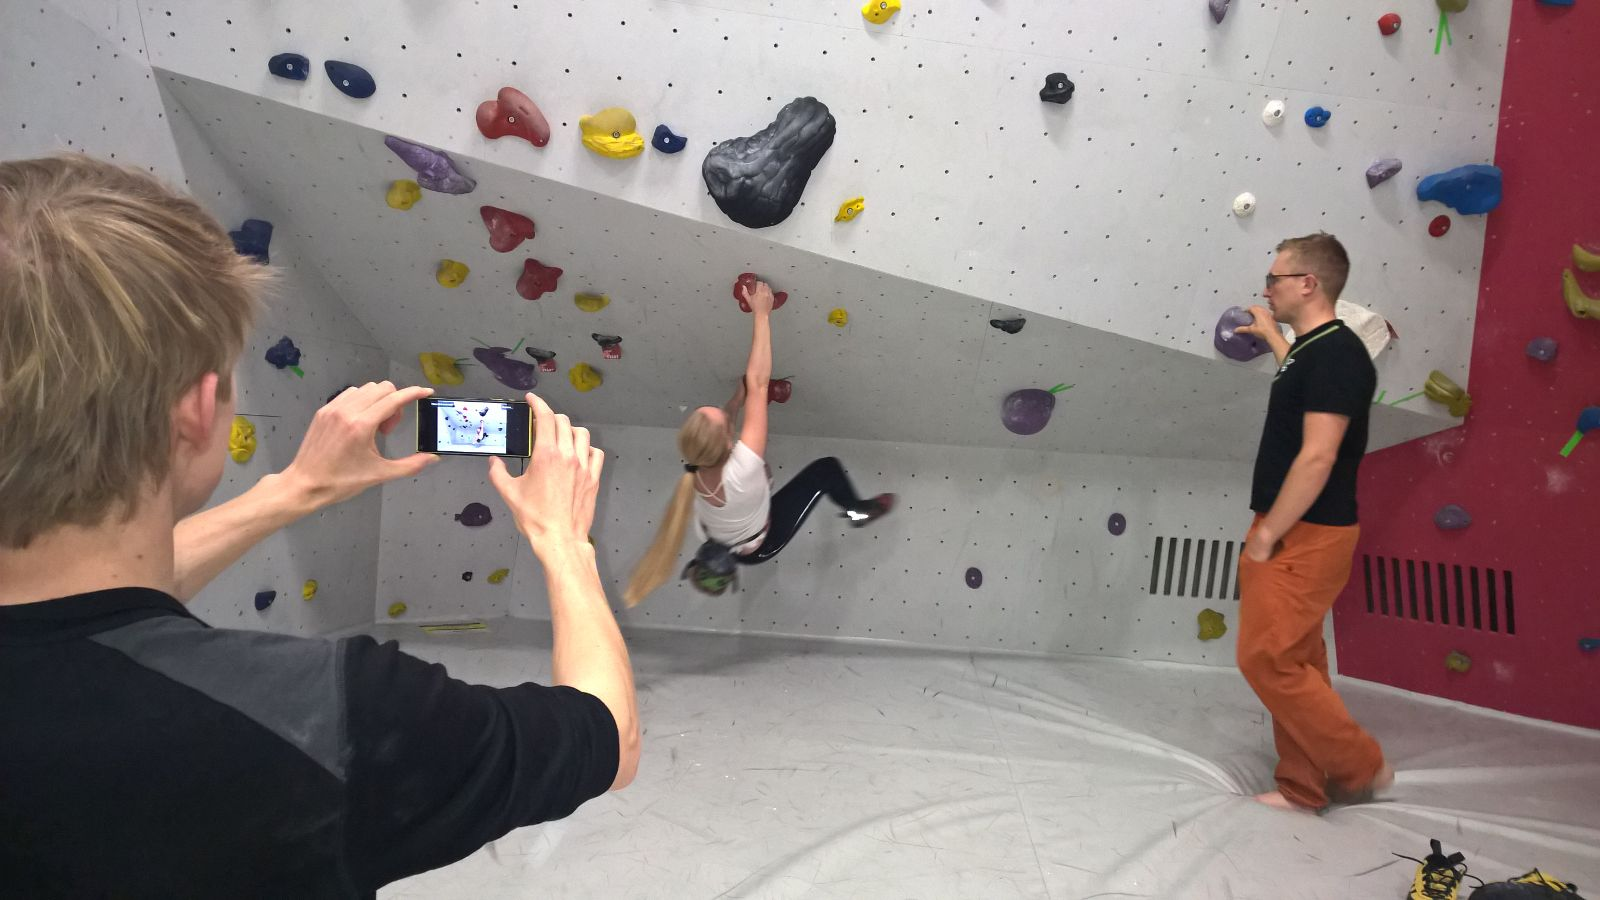
\includegraphics[width=\textwidth]{figures/images/Live-Video.jpg}
        \caption{A camera operator with a smartphone, and climber, wearing a Google Glass.}
        \label{fig:live-video-action}
    \end{subfigure}
    \caption{The live video setup, utilizing a smartphone and a pair of smart glasses.}
    \label{fig:live-video}
\end{figure}


The system chosen uses two hardware components. The camera operator uses a smartphone to capture video signals which are displayed using a pair of smart glasses. Both are consumer products and fulfill the requirement for the system being minimally invasive and easy to set up. The aspect of latency will be discussed in detail later when explaining the software. A Sony Xperia Z5 Compact\footnote{\url{http://www.gsmarena.com/sony_xperia_z5_compact-7535.php}} running Android 6.0.1, and a Google Glass\footnote{\url{https://support.google.com/glass/answer/3064128}} running Android 4.4.4 (\figref{fig:google-glass}) as well as a Vuzix M100\footnote{\url{https://www.vuzix.com/Products/m100-smart-glasses}} running Android 4.0.4 have been used as hardware components. The software to capture and provide live video matrial is an app called IP Webcam\footnote{\url{https://play.google.com/store/apps/details?id=com.pas.webcam}}, which works like a regular IP camera\footnote{\url{https://en.wikipedia.org/wiki/IP_camera}}. It delivers images through HTTP as a stream of multipart/x-mixed-replace\footnote{\url{https://en.wikipedia.org/wiki/MIME\#Mixed-Replace}} encoded JPEG images. Smartphone and smart glasses are connected over WiFi, using the smartphone as a router to establish a network.

For the client side there was no app available to view IP camera video streams, especially not for smart glasses. The first draft was based on an app called SimpleJPEGView\footnote{\url{https://bitbucket.org/neuralassembly/simplemjpegview}} which was then optimized for the limited resources available on smart glasses. As a first step, reading images from the input stream was implemented utilizing the well-tested Knuth-Morris-Pratt search algorithm from Twitters Elephant Bird library\footnote{\url{https://github.com/twitter/elephant-bird/blob/master/core/src/main/java/com/twitter/elephantbird/util/StreamSearcher.java}} that was modified, so it could also write bytes, read from the input stream into a direct buffer. Writing relevant bytes in a direct buffer immediately, saves expensive memory copies, which speeds up decompressing the JPEG written into it. Decompression is delegated to the also well-tested library TurboJPEG\footnote{\url{http://www.libjpeg-turbo.org/About/TurboJPEG}}, which is controlled by a piece of native C++ code, again to reduce the need for memory copies. With this setup, a $320 \times 240$ pixel image took \SIrange{20}{25}{\ms} to read and \SIrange{3}{7}{\ms} to decompress, resulting in an average processing time of \SI{30}{\ms} per image. That enables frame rates of up to 30 frames per second. However, the overall latency for the video signal to travel from the smartphone to the smart glasses is \SI{100}{\ms} in average.

\begin{figure}[h]
    \centering
    \begin{subfigure}[b]{0.49\columnwidth}
        \centering
        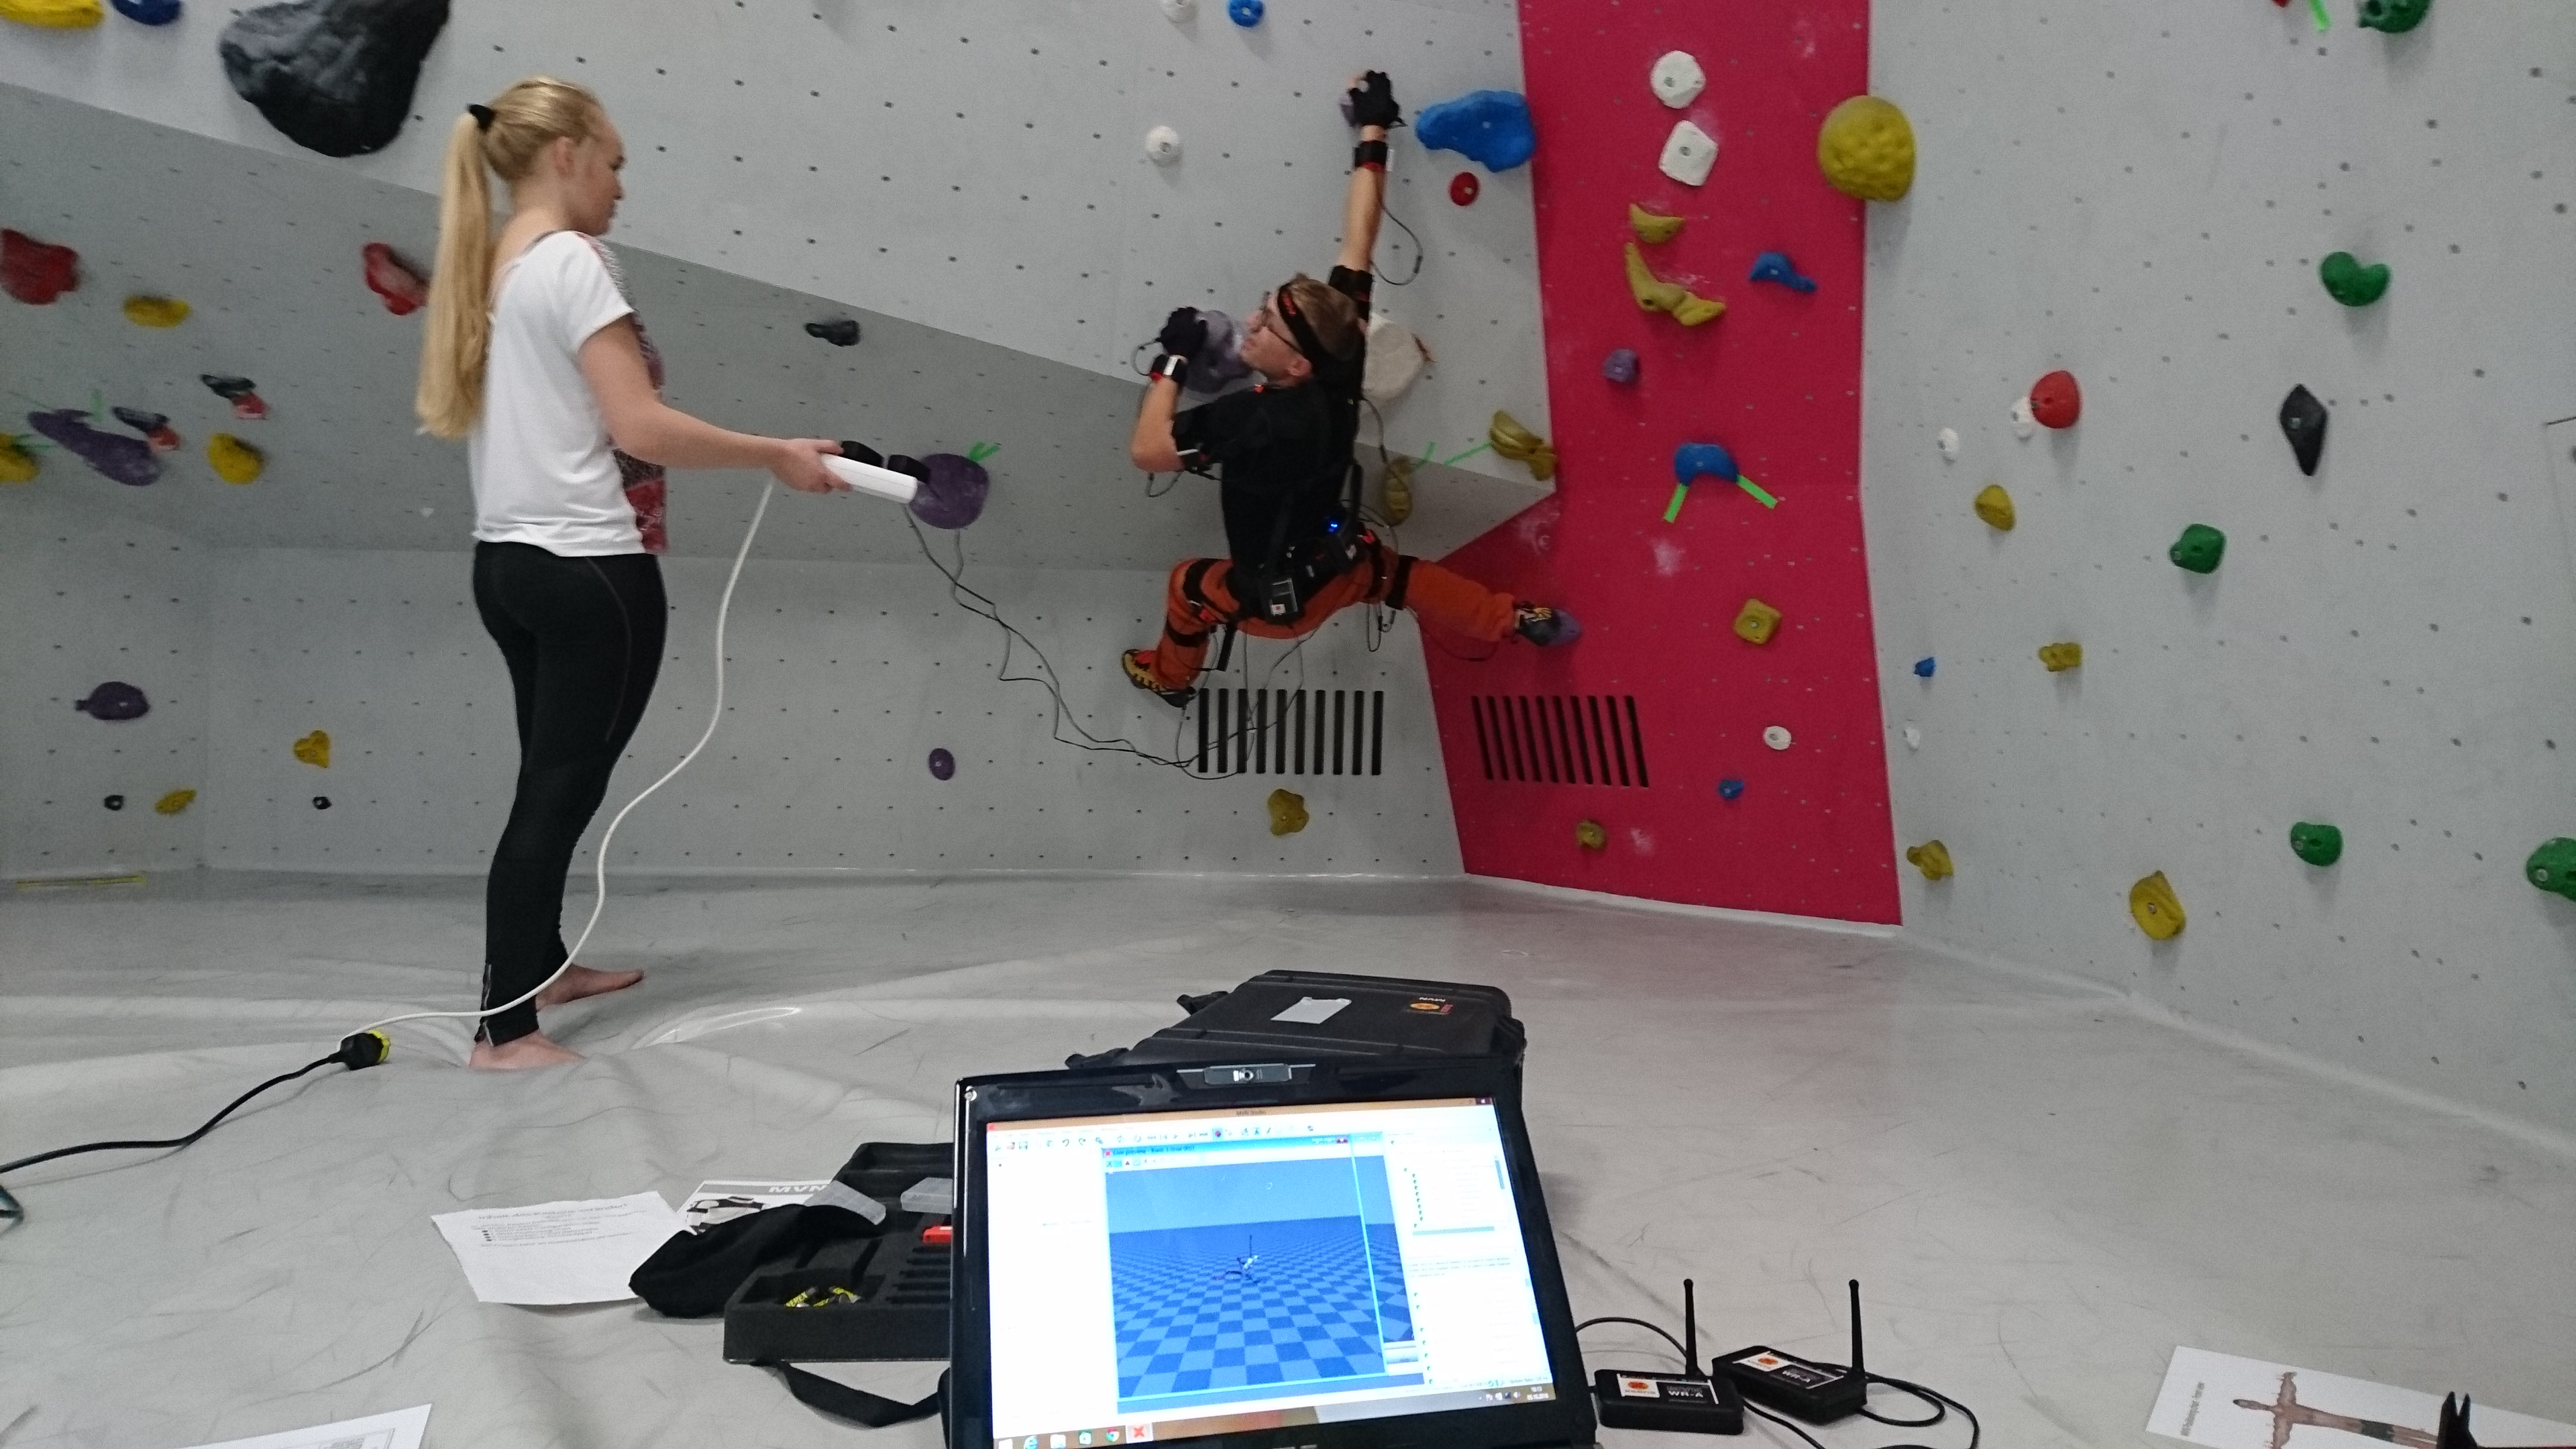
\includegraphics[width=0.96\textwidth]{figures/images/Moven-In-Action.jpg}
        \caption{A participant climbing, wearing the XSense MVN Bio Mech suit.} \label{fig:mvn-in-use}
    \end{subfigure}
    \hspace*{\fill}
    \begin{subfigure}[b]{0.49\columnwidth}
        \centering
        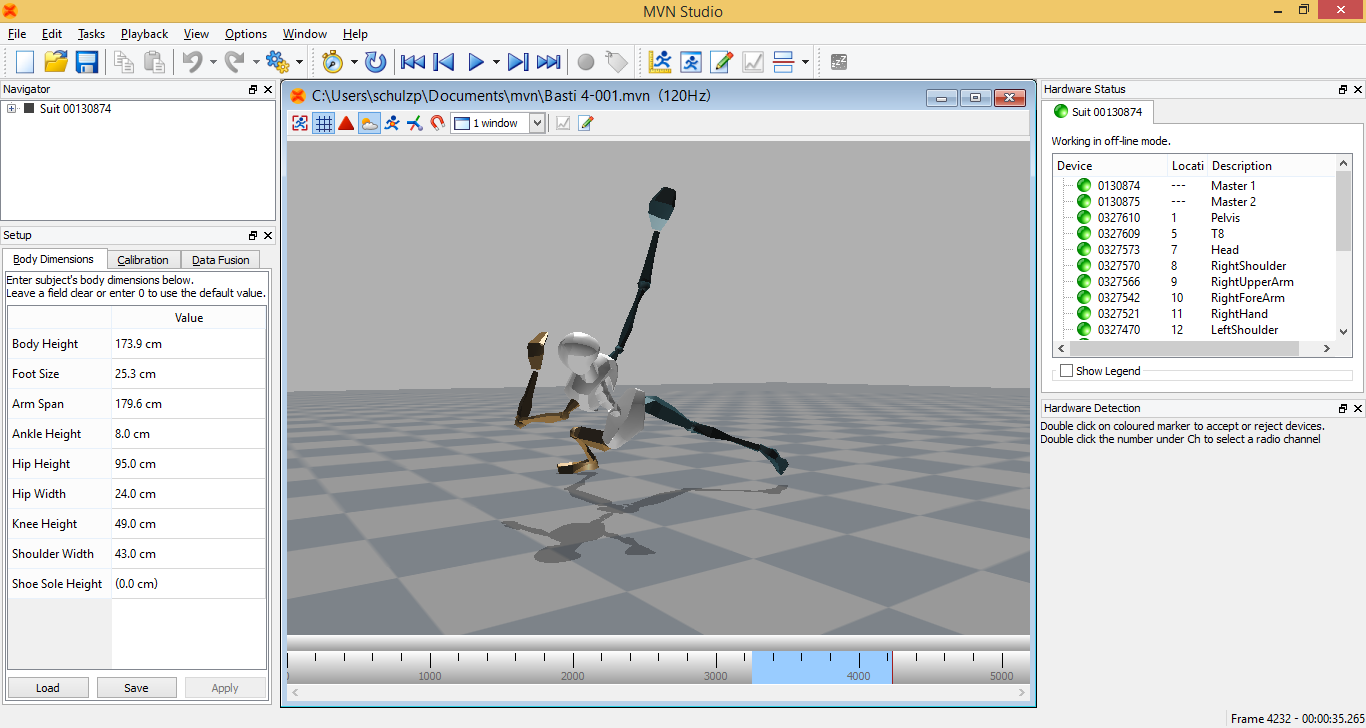
\includegraphics[width=\textwidth]{figures/images/Moven-Screenshot.png}
        \caption{A screenshot of XSense MVN Studio, showing a replay of a paricipant while climbing.} \label{fig:mvn-screenshot}
    \end{subfigure}
    \caption{The XSense MVN System being used to capture climbing movements.}
    \label{fig:mvn-suit}
\end{figure}


For the second condition, a recording of movements had to be recorded in 3D. This was achieved by using well-tested motion capture technology, namely the Xsense MVN System, which is a markerless tracking system. The participant wears a set of 17 connected IMUs which broadcasts signals at \SI{120}{\Hz}. The transmission takes place wirelessly to a laptop running Xsense MVN Studio that is merging the sensor output and mapping it into movements of a humanoid model, \cf \figref{fig:mvn-suit}. 

\subsection{Results}

After each experiment the participating climbers filled in a questionnaire regarding the perceived usability of the system. It was explained to them that the tested system is still an early prototype and  they were free to imagine an advanced version of it when evaluating.

\paragraph{Perceived Usability}

The questions of the final SUS questionnaire are divided in two parts, where the first part consists of the standard questions \autocite{susgov} 1-5, and 8 and 9. For the second part, three questions were added to the original set of questions, which target the climbing context more specifically.

\begin{figure}[h]
    \centering
    \begin{subfigure}[b]{\textwidth}
        \centering
        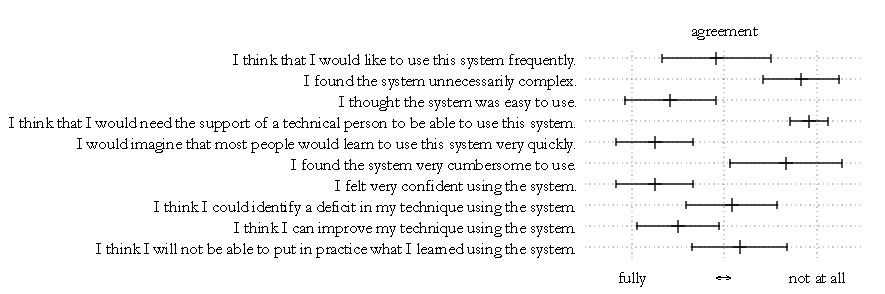
\includegraphics[width=\textwidth]{figures/plots/sus-glasses.pdf}
        \caption{First condition, the smart glasses. 6 Participants}
        \label{fig:sus-glasses}    
    \end{subfigure}
    \begin{subfigure}[b]{\textwidth}
        \centering
        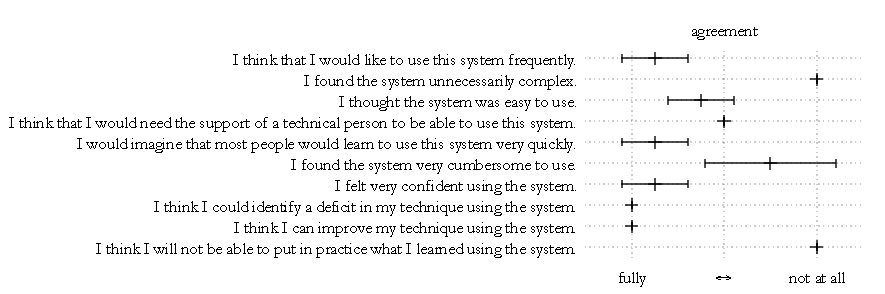
\includegraphics[width=\textwidth]{figures/plots/sus-mvn.pdf}
        \caption{Second condition, the motion tracking suit. 2 Participants}
        \label{fig:sus-mvn}
    \end{subfigure}
    \caption{SUS questions and results. A higher color saturation means more answers.}
    \label{fig:sus-results}
\end{figure}


At first glance, the majority of the participants agrees that using the smart glasses is not to complex, \cf \figref{fig:sus-glasses}. However, when asked for the perceived benefit of the system to their climbing skills --- the last three questions --- those questioned are less polarized. 

The results for the second condition are quite similar, \cf \figref{fig:sus-mvn}. In contrast to the results for the smart glasses, the participants are more convinced of the actual benefit of this approach. At the same time, using a motion tracking suit is not perceived as easy as wearing smart glasses.

\paragraph{Feedback Given by Participants}

Within the final questionnaire, the participants were given the opportunity to state what they dislike or would like to improve about the system they just tested. The experimenter also asked them about this. Most of the feedback regards the first condition --- the smart glasses.

Two out of six participants found the Vuzix glasses were fitting to loose. Only one participant complained about the display blocking the view, whereas all the others considered this not being a problem when explicitly asked about that. Going beyond the hardware, another participant explained that it was difficult to mentally take the position of the camera and switch to that perspective. A third of the respondents considered the display to be too small and that it was hard to keep an eye on it while climbing. Especially, when trying a tiring move, all questioned reported that they found it difficult to concentrate on interpreting the image of themselves --- however, five out of six had no trouble checking their pose while staying in a resting climbing position. One participant in particular claimed he could identify an insufficient pose through the video image and, after a hint given by a trainer, he found it helpful to immediately see the benefit achieved by moving in a different way. Yet another participant guessed that it might take some time to get used to the system before actually deriving benefit from the additional visual input.

The second condition was only tested by two participants, who were questioned afterwards in the same fashion as for the first condition. Both trainees, one female and one male, reportedly liked the replay of the virtual 3D model imitating their movements, \cf \figref{fig:mvn-screenshot}. Especially, panning around the 3D model during replay was considered highly informative, since it made effects of different poses very clear. As it were, both questioned found it too awkward putting on the suit, which renders the system less usable in their eyes.
\section{Discussion}

The study lead to unexpected results: On the one hand, smart glasses showing a live video are easy to use, but the benefit is challenged. On the other hand, a 3D visualization of movements --- despite its cumbersome production --- is considered highly insightful. The results of the smart glasses correspond to those of \textcite{Kosmalla:2016:CIP:2858036.2858562}, who found out that it is harder for climbers to process visual input rather than other inputs while climbing. Apart from that, the approach of using live video was new to all participants, in contrast to the post hoc analysis, which they are already familiar with, due to the previous utilization of video analysis.

Yet, value should be attached carefully to the results of this study, for several reasons. First, the number people who participated in the study is extremely low, which increases the risk of the probe not being representative. Second, all of the participants knew the experimenter previous to the tests, which may lead to a bias in the results. Third, it is impossible to say if either of the tested conditions have a measurable effect on the imagery skills of the participants, since the gathered data does not allow such a conclusion. Finally, none of the participants have worked as trainers before and are therefore most likely not familiar with interpreting recordings.
\section{Conclusion}

As part of this study, trainers have been interviewed to find out how they coach trainees, how technology is used to support the training, and how technology might be put in use further on. These interviews lead to the insight that imagery is an important skill in climbing, which enables those who master it to plan strategically and climb efficiently.

Two concepts to support learning imagery were tested for their perception and acceptance in a small study. Both, smart glasses showing live video, as well as motion capturing for a post hoc analysis were received well. The results of the study show that the expected benefit of using either system differs in favor of the post hoc analysis. However, the results are not meaningful as the sample of participating climbers is flawed because of its small size.

This study introduced two new approaches --- in situ self-observation and post hoc motion capture replay ---to support climbing training, which can be examined more extensively. Further research is needed, for example, to look into the actual effect that each of the approaches has on the imagery skills of climbers and if the approaches offer a greater benefit than conventional video analysis. 
